% ABOUTME: Results: synthesis, CPI and IPC, execution time, and why the speedup is what it is.
% ABOUTME: Owner: Husain (review every number against results/, rerun make synth perf to check).
\section{Results}
\label{sec:results}

\subsection{Setup}
Synthesis uses Yosys \cite{yosys} (\texttt{synth\_ecp5}) and place and route
uses nextpnr \cite{nextpnr} for a Lattice ECP5 LFE5U-25F, speed grade 6,
package CABGA381 \cite{ecp5}, the FPGA on boards such as the ULX3S. Each CPU
sits in a small top level that shows the last value written back on eight
LEDs, so no logic can be optimised away, and runs the bubble sort program from
its instruction ROM. nextpnr results depend on a random placement seed, so
each design is placed with five seeds and we report the median.

\subsection{Synthesis}
Table~\ref{tab:synth} gives the results. The pipeline registers add about
260 flip-flops. Without forwarding the pipeline's clock is 1.94 times the
single-cycle clock; with forwarding it is 1.43 times, because the forwarding
comparators and muxes sit in front of the ALU and the branch comparator, on
the path that ends in the flush of IF/ID and ID/EX.

\begin{table}[t]
\centering
\caption{ECP5 results, median of five seeds (LUT memories)}
\label{tab:synth}
\small
\setlength{\tabcolsep}{3pt}
\begin{tabular}{@{}lrrrr@{}}
\toprule
CPU & Logic cells & FFs & Fmax (MHz) & Range \\
\midrule
Single-cycle & 2076 & 43 & 58.75 & 57.7--60.2 \\
Pipeline, no fwd & 2137 & 299 & 113.86 & 110.1--115.5 \\
Pipeline, fwd & 2765 & 308 & 83.89 & 83.6--86.9 \\
\bottomrule
\end{tabular}
\end{table}

\textbf{Memory style matters.} When Yosys may use the FPGA's block RAM, it
notices that each memory feeds a pipeline register and folds that register
into the block RAM. This is legal and saves flip-flops, but an ECP5 block RAM
has a 5.6\,ns clock-to-output delay, so the ID stage and the MEM/WB forwarding
path then start with 5.6\,ns already spent. With block RAM the three designs
reach only 42.2, 72.2 and 59.1\,MHz (Fig.~\ref{fig:fmax}). We therefore place
both 256 word memories in LUTs, where every pipeline register stays a real
flip-flop and the stage boundaries in the RTL are the stage boundaries in the
hardware. Larger memories would need block RAM and an extra pipeline stage or a
registered address, as real processors do.

\begin{figure}[t]
\centering
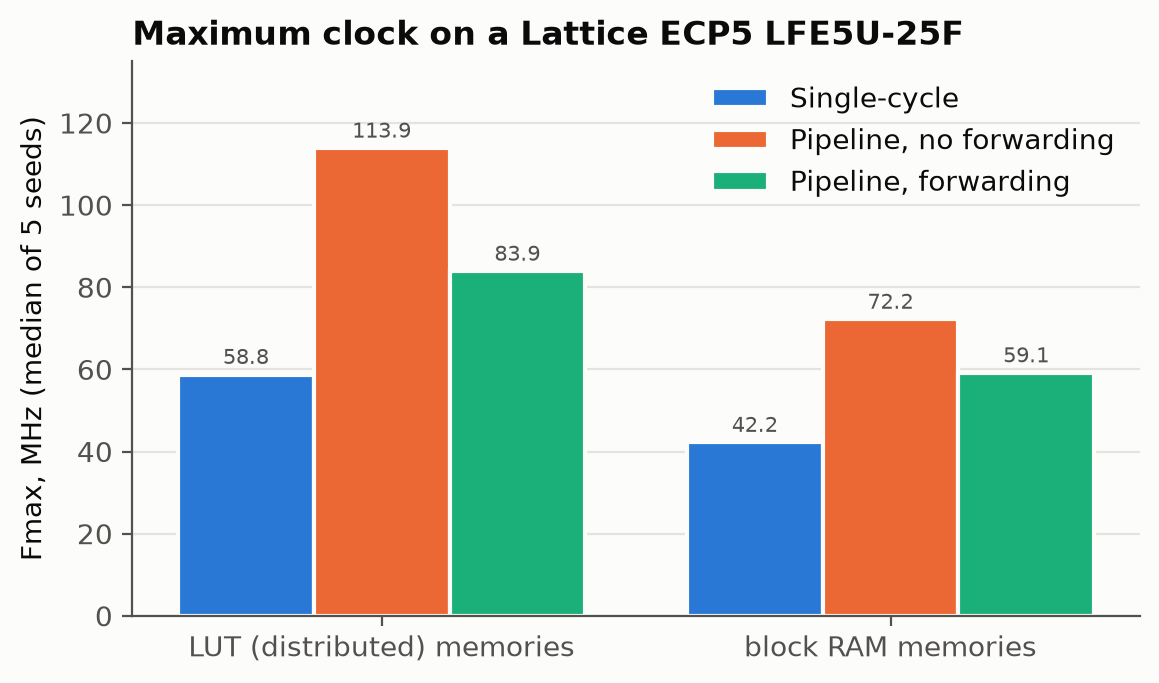
\includegraphics[width=\columnwidth]{fmax.png}
\caption{Fmax of each CPU with LUT memories and with block RAM.}
\label{fig:fmax}
\end{figure}

\subsection{CPI and IPC}
Table~\ref{tab:cpi} lists CPI and IPC for every benchmark. The single-cycle
CPU has CPI 1.00 by construction. Fig.~\ref{fig:breakdown} splits each
pipelined CPI with (\ref{eq:cycles}). Without forwarding, data hazard stalls
dominate: \texttt{dep\_chain}, where each instruction needs the one before
it, stalls for 241 cycles over 163 instructions. Forwarding removes every
one of those stalls; what remains are load-use stalls (66 in bubble sort, one
per inner iteration, and 16 in the array sum) and branch flushes. Every loop
iteration ends in a taken branch, so with loop bodies of six to ten
instructions the flushes alone add 0.23 to 0.35 to CPI. The four fill cycles
are negligible for programs of 86 instructions or more.

\begin{table}[t]
\centering
\caption{CPI (IPC in brackets) per benchmark}
\label{tab:cpi}
\small
\setlength{\tabcolsep}{4pt}
\begin{tabular}{@{}lrrr@{}}
\toprule
Benchmark ($N$) & Single & Pipe, no fwd & Pipe, fwd \\
\midrule
bubble\_sort (591) & 1.00 & 2.07 (0.48) & 1.45 (0.69) \\
dep\_chain (163) & 1.00 & 2.74 (0.37) & 1.26 (0.80) \\
fibonacci (215) & 1.00 & 1.71 (0.59) & 1.29 (0.78) \\
indep\_ops (162) & 1.00 & 1.51 (0.66) & 1.26 (0.79) \\
sum\_array (86) & 1.00 & 2.16 (0.46) & 1.58 (0.63) \\
\bottomrule
\end{tabular}
\end{table}

\begin{figure*}[t]
\centering
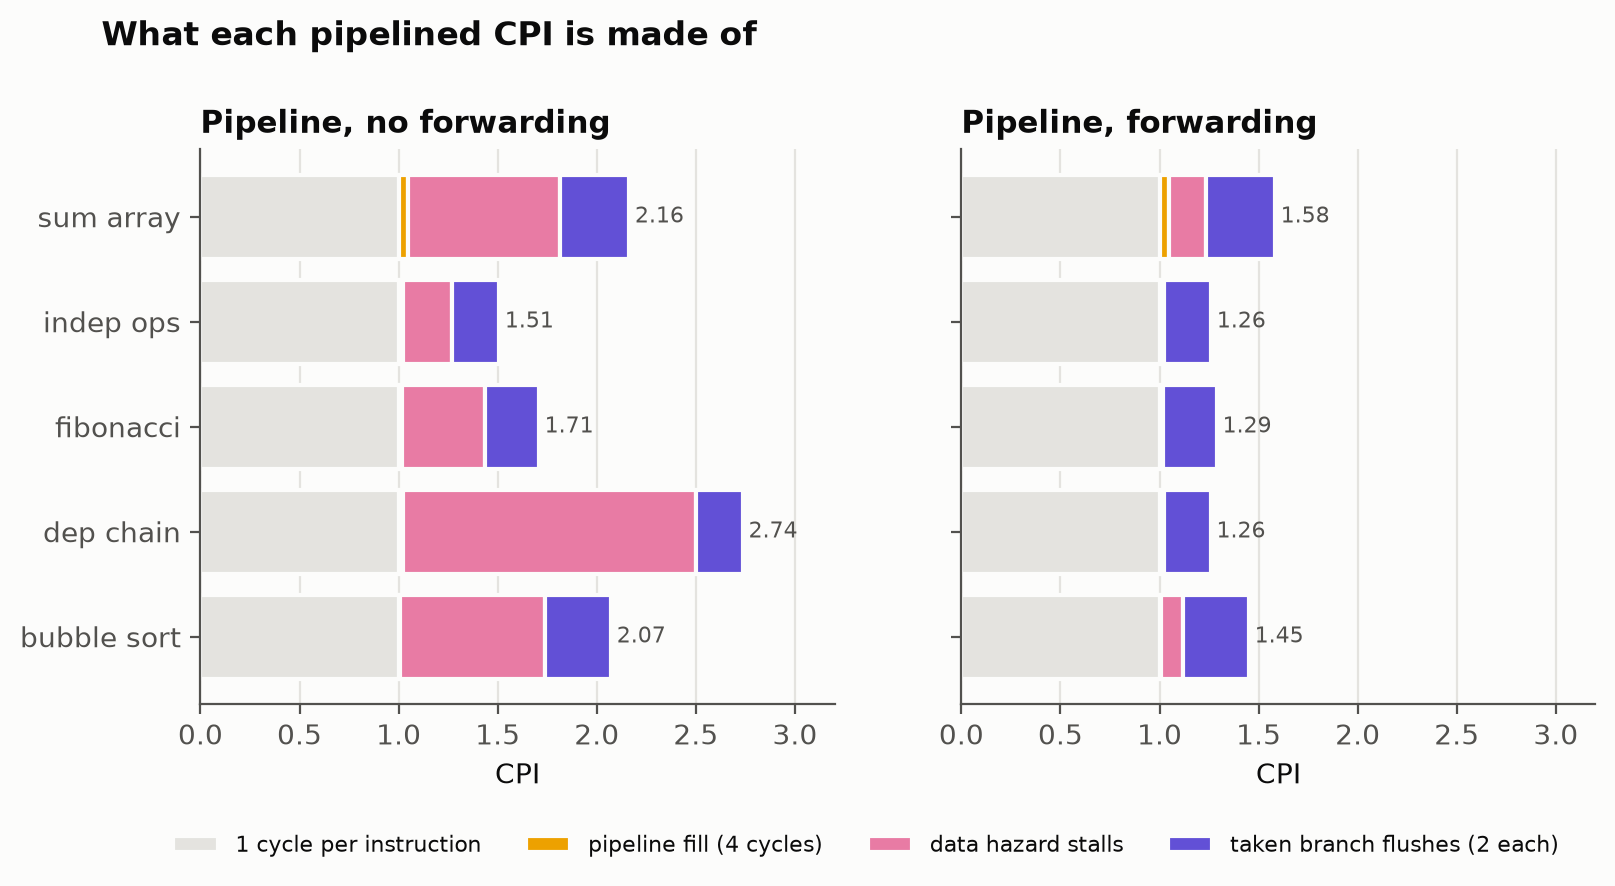
\includegraphics[width=0.85\textwidth]{cpi_breakdown.png}
\caption{Where the pipelined cycles go: one cycle per instruction plus fill,
data hazard stalls and taken branch flushes, per benchmark.}
\label{fig:breakdown}
\end{figure*}

\subsection{Execution time}
Combining cycles with Fmax gives execution time and the speedup over the
single-cycle CPU (Fig.~\ref{fig:speedup}). Equation (\ref{eq:speedup}) makes
the outcome predictable: the forwarding pipeline wins only when its CPI is
below 1.43, and the pipeline without forwarding only when its CPI is below
1.94. With forwarding, \texttt{dep\_chain}, \texttt{fibonacci} and
\texttt{indep\_ops} (CPI 1.26 to 1.29) run 1.11 to 1.14 times faster, while
bubble sort and the array sum (CPI 1.45 and 1.58) run slightly slower. The
pipeline without forwarding has the best clock and wins on code with few
dependences (\texttt{indep\_ops}, 1.29 times), but loses badly on dependent
chains (0.71 times). Forwarding therefore trades a 26\,\% slower clock for a
much more predictable CPI: its worst case is 0.90, against 0.71 without it.

\begin{figure}[t]
\centering
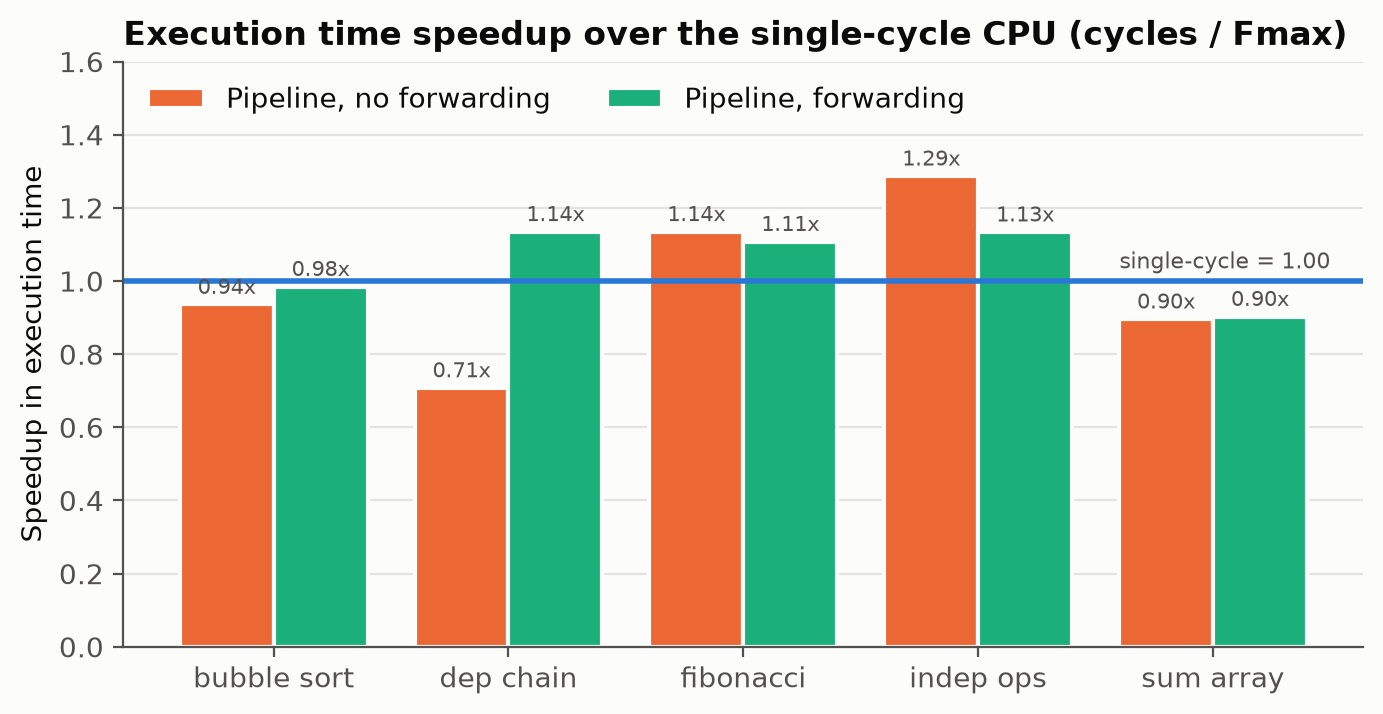
\includegraphics[width=\columnwidth]{speedup.png}
\caption{Execution time speedup over the single-cycle CPU (cycles divided by
Fmax). Above 1 the pipeline is faster.}
\label{fig:speedup}
\end{figure}

\subsection{Why not five times faster}
An ideal five-stage pipeline would have a clock five times faster and
CPI 1. Ours falls short on both counts. First, the stages are not balanced:
the data memory read alone takes 8.0 of the single-cycle CPU's 17.0\,ns, and
EX holds the ALU, the forwarding muxes and the branch decision, so the
longest stage is about half of the single-cycle path, not a fifth. Second,
the branch penalty of two cycles per loop iteration costs a quarter to a
third of a cycle per instruction. The clearest next steps are therefore a
branch predictor or resolving branches in ID (one cycle penalty instead of
two), and rebalancing the slowest stages: EX, whose ALU and forwarding path
set the clock in both pipelines, and MEM, whose 8\,ns memory read is close
behind.
